\chapter{Notes on Gaussian Process Time Series Models}\label{app:gpNARX}

Gaussian processes provide a systematic and flexible framework for probabilistic inference in machine learning. 
Their formulation is general and their existence is dependent on two key conditions outlined in \cref{sec:osaGPmethod} 
which we restate here.

For any input space $x \in \mathcal{X}$, a real valued scalar GP (\cref{eq:gpformulationapp}) can be created given two functions.

\begin{enumerate}
    \item A mean function $m: \mathcal{X} \longrightarrow \mathbb{R}$.
    \item A symmetric positive definite covariance function $K: \mathcal{X} \times \mathcal{X} \longrightarrow \mathbb{R}^{+}$ \citep[ch.~1\&2]{Berlinet2004}.
\end{enumerate}    

\begin{equation}\label{eq:gpformulationapp}
    f(x) \sim \mathcal{GP}(m(x), K(x, x'))
\end{equation}

It is important to note that there are no restrictions placed on the input space $\mathcal{X}$ in the definition of GPs. The inputs 
can be continuous, discrete or having complex structure. \citet[ch.~4, sec.~4.4]{Rasmussen:2005:GPM:1162254} gives some examples of 
covariance funtions defined over the space of strings (sequences of characters drawn from a finite alphabet) and note that it is indeed 
possible to construct covariance functions over structured objects such as trees and general graphs. 

Gaussian process time series modelling has associated with it a rich body of work \citep{turner2012gaussian,frigola2016bayesian}. There 
are two ways in which GP models can be applied to time series data: \begin{enumerate*} \item explicit time \& \item implicit time \end{enumerate*}

\section*{Explicit vs Implicit Representation}

Depending on whether or not time appears directly in the inputs space of a GP, we can classify a GP time series model as explicit or 
imlicit respectively. Notationally, explicit and implicit time GP formulations are shown in \cref{eq:gpExplicit} and \cref{eq:gpImplicit} respectively.

\begin{align}
    y(t) &\sim \mathcal{GP}(m(t), K(t, s)) \label{eq:gpExplicit}\\
    y(t) &\sim \mathcal{GP}(m(\mathbf{x}(t)), K(\mathbf{x}(t), \mathbf{x}(s))) \label{eq:gpImplicit}
\end{align}

In the explicit time GP model, the mean and covariance of the process are functions of the continuous time coordinate $t$. On the other hand 
in implicit time GP models, the mean and covariance are functions of some state space $\mathbf{x}_t$. This key difference has significant 
implications for the system trajectories and uncertainty characteristics.


\subsection*{GP-AR \& GP-ARX as Simulation Models}

\begin{figure}
    \centering
    \noindent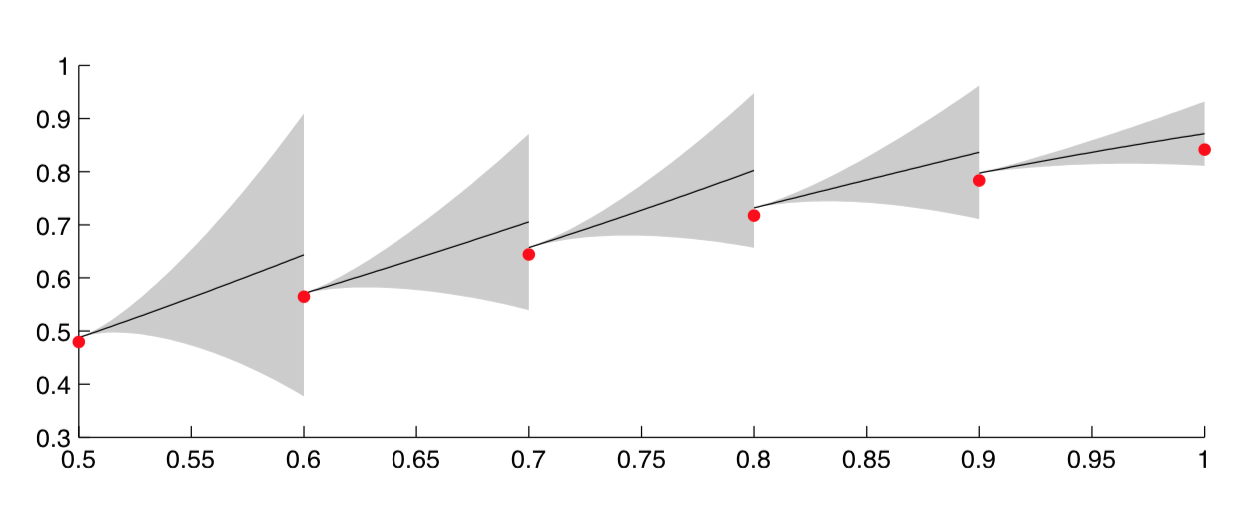
\includegraphics[width=0.75\textwidth]{gpar.png}
    \caption{Successive simulation of the GP-AR model}
    \label{fig:gparDiag}
\end{figure}


\begin{align}
    y_0 &= u \label{eq:gpARInit}\\
    y_t \rvert y_{t-1} &\sim \mathcal{N}(m(y_{t - 1}), K(y_{t - 1}, y_{t - 1})) \label{eq:gpARProp}
\end{align}

\subsubsection*{Exogenous Inputs}



\subsection*{Relationship with Time Series Models : $\mathrm{AR}(p)$}

Due to the abstract nature of GPs, they actually generalize some popular time series models. Consider $\mathrm{AR}(p)$, the family of discrete 
auto-regressive time series models shown in \cref{eq:ARp}. At each time step, the systems state $Y_t$ is determined by a linear combination 
of $p$ previous system states $Y_{t-1}, \cdots, Y_{t-p}$ added to Gaussian noise.  

\begin{align}
    Y_t &= \sum^{p}_{k = 1}{\phi_{k}Y_{t-k}} + Z_t \label{eq:ARp} \\
    Z_t &\sim \mathcal{N}(0, \sigma^{2}_{\varepsilon})
\end{align}

We can write \cref{eq:ARp} in probabilistic form as: 
\begin{equation*}
    Y_t \rvert Y_{t-1}, \cdots, Y_{t-p} \sim \mathcal{N}(\sum^{p}_{k = 1}{\phi_{k}Y_{t-k}}, \sigma^{2}_{\varepsilon})
\end{equation*}



